\chapter{Numeros reales y herramientas numericas}

\begin{theorybox}{Trazabilidad del capitulo}
Este capitulo desarrolla las secciones \texttt{C01.S01-C01.S07} de la matriz de cobertura a
partir de \texttt{sources/Relacion tema 1.pdf}. El objetivo es convertir las tipologias del
tema 1 en procedimientos reconocibles, con ejemplo resuelto, ejercicios guiados y practica
graduada.
\end{theorybox}

\section{[C01.S01] Clasificacion de numeros y conjuntos numericos}

\subsection*{Objetivos de aprendizaje}
\begin{itemize}
  \item Identificar el conjunto mas pequeno al que pertenece un numero.
  \item Distinguir naturales, enteros, racionales, irracionales y reales.
\end{itemize}

\subsection*{Prerrequisitos}
\begin{itemize}
  \item Leer fracciones, decimales y radicales sencillos.
\end{itemize}

\begin{theorybox}{Idea minima}
\[
\mathbb{N}\subset \mathbb{Z}\subset \mathbb{Q}\subset \mathbb{R}.
\]
Los irracionales son los reales que no son racionales. Un decimal exacto o periodico es
racional. Una raiz como \(\sqrt{49}\) puede simplificarse y cambiar de conjunto.
\end{theorybox}

\begin{methodbox}{Como reconocer y resolver}
\begin{enumerate}
  \item Simplifica el numero si aparece una raiz o una operacion.
  \item Decide si el resultado es natural, entero, racional o irracional.
  \item Da, si se pide, el conjunto mas pequeno al que pertenece.
\end{enumerate}
\end{methodbox}

\begin{solvedexample}{[EX-C01.S01-01] Clasificar con el conjunto mas pequeno}
Clasifica los numeros \(-7\), \(0.125\), \(\sqrt{2}\) y \(\sqrt{49}\).

\textbf{Desarrollo.}
\begin{itemize}
  \item \(-7\) es entero, asi que el conjunto mas pequeno es \(\mathbb{Z}\).
  \item \(0.125\) es un decimal exacto, luego es racional: \(\mathbb{Q}\).
  \item \(\sqrt{2}\) no puede escribirse como fraccion exacta, luego es irracional.
  \item \(\sqrt{49}=7\), asi que pertenece a \(\mathbb{N}\).
\end{itemize}

\textbf{Respuesta final.}
\[
-7\in\mathbb{Z},\qquad 0.125\in\mathbb{Q},\qquad \sqrt{2}\in\mathbb{R}\setminus\mathbb{Q},
\qquad \sqrt{49}\in\mathbb{N}.
\]
\end{solvedexample}

\begin{commonerror}{No simplificar antes de clasificar}
Ver \(\sqrt{49}\) y marcarlo como irracional es un error frecuente. Antes de clasificar hay que
simplificar: \(\sqrt{49}=7\), que es natural.
\end{commonerror}

\begin{guidedexercise}{[GX-C01.S01-01] Clasificacion de un entero oculto}
Clasifica \(-\dfrac{\sqrt{16}}{2}\).

\textbf{Pista 1.} Empieza por simplificar la raiz.

\textbf{Pista 2.} El resultado final es un entero.
\end{guidedexercise}

\begin{shortanswer}{[GX-C01.S01-01]}
\(-\dfrac{\sqrt{16}}{2}=-2\), luego pertenece a \(\mathbb{Z}\).
\end{shortanswer}

\begin{fullsolution}{[GX-C01.S01-01]}
\[
-\frac{\sqrt{16}}{2}=-\frac{4}{2}=-2.
\]
El conjunto mas pequeno al que pertenece es \(\mathbb{Z}\).
\end{fullsolution}

\begin{guidedexercise}{[GX-C01.S01-02] Clasificacion de un decimal periodico}
Clasifica \(0.\overline{3}\).

\textbf{Pista 1.} Todo decimal periodico es racional.
\end{guidedexercise}

\begin{shortanswer}{[GX-C01.S01-02]}
\(0.\overline{3}\in\mathbb{Q}\).
\end{shortanswer}

\begin{fullsolution}{[GX-C01.S01-02]}
El numero \(0.\overline{3}\) es un decimal periodico, asi que puede escribirse como fraccion:
\[
0.\overline{3}=\frac{1}{3}.
\]
Por tanto, pertenece a \(\mathbb{Q}\).
\end{fullsolution}

\subsection*{Practica autonoma graduada}
\begin{exercise}{[PX-C01.S01-01] Clasifica \(\sqrt{7}\).}
\end{exercise}
\begin{exercise}{[PX-C01.S01-02] Clasifica \(\dfrac{5}{4}\).}
\end{exercise}
\begin{exercise}{[PX-C01.S01-03] Clasifica \(-\sqrt{81}\).}
\end{exercise}
\begin{exercise}{[PX-C01.S01-04] Clasifica \(0\).}
\end{exercise}
\begin{exercise}{[PX-C01.S01-05] Clasifica \(2-\sqrt{4}\).}
\end{exercise}
\begin{exercise}{[PX-C01.S01-06] Clasifica \(3.1415\).}
\end{exercise}

\begin{shortanswer}{C01.S01 practica autonoma}
\begin{enumerate}[label=\textbf{PX-C01.S01-\arabic*:}, leftmargin=*]
  \item \(\mathbb{R}\setminus\mathbb{Q}\)
  \item \(\mathbb{Q}\)
  \item \(\mathbb{Z}\)
  \item \(\mathbb{Z}\)
  \item \(\mathbb{Z}\)
  \item \(\mathbb{Q}\)
\end{enumerate}
\end{shortanswer}

\begin{fullsolution}{C01.S01 practica autonoma}
\begin{enumerate}[label=\textbf{PX-C01.S01-\arabic*:}, leftmargin=*]
  \item \(\sqrt{7}\) no es raiz exacta, luego es irracional.
  \item \(\frac{5}{4}\) es una fraccion de enteros con denominador no nulo, luego es racional.
  \item \(-\sqrt{81}=-9\), luego es entero.
  \item \(0\) pertenece a \(\mathbb{Z}\).
  \item \(2-\sqrt{4}=2-2=0\), luego pertenece a \(\mathbb{Z}\).
  \item \(3.1415\) es decimal exacto, luego es racional.
\end{enumerate}
\end{fullsolution}

\section{[C01.S02] Decimales y fraccion generatriz}

\subsection*{Objetivos de aprendizaje}
\begin{itemize}
  \item Distinguir decimales exactos, periodicos puros y periodicos mixtos.
  \item Hallar la fraccion generatriz de un decimal.
\end{itemize}

\subsection*{Prerrequisitos}
\begin{itemize}
  \item Operar con ecuaciones lineales sencillas.
\end{itemize}

\begin{theorybox}{Idea minima}
Un decimal exacto siempre es racional. Tambien lo es un decimal periodico. Para hallar su
fraccion generatriz se usa una ecuacion: se multiplica por potencias de \(10\) hasta alinear la
parte periodica y luego se resta.
\end{theorybox}

\begin{methodbox}{Como reconocer y resolver}
\begin{enumerate}
  \item Decide si el decimal es exacto, periodico puro o mixto.
  \item Si es exacto, escribe el numero sin coma sobre una potencia de \(10\).
  \item Si es periodico, llama \(x\) al numero y alinea el periodo con potencias de \(10\).
  \item Resta las ecuaciones y despeja \(x\).
\end{enumerate}
\end{methodbox}

\begin{solvedexample}{[EX-C01.S02-01] Fraccion generatriz de un decimal mixto}
Halla la fraccion generatriz de \(1.2\overline{3}\).

\textbf{Desarrollo.} Sea \(x=1.2\overline{3}\).
\[
10x=12.\overline{3},
\qquad
100x=123.\overline{3}.
\]
Restamos:
\[
100x-10x=123.\overline{3}-12.\overline{3}=111.
\]
Entonces
\[
90x=111
\qquad\Longrightarrow\qquad
x=\frac{111}{90}=\frac{37}{30}.
\]

\textbf{Respuesta final.}
\[
1.2\overline{3}=\frac{37}{30}.
\]
\end{solvedexample}

\begin{commonerror}{Mover la coma sin alinear el periodo}
En un decimal mixto no basta con multiplicar una sola vez por \(10\). Hay que conseguir que la
parte periodica quede igual en las dos expresiones antes de restar.
\end{commonerror}

\begin{guidedexercise}{[GX-C01.S02-01] Periodico puro}
Halla la fraccion generatriz de \(0.\overline{18}\).

\textbf{Pista 1.} El periodo tiene dos cifras.
\end{guidedexercise}

\begin{shortanswer}{[GX-C01.S02-01]}
\[
0.\overline{18}=\frac{2}{11}.
\]
\end{shortanswer}

\begin{fullsolution}{[GX-C01.S02-01]}
Sea \(x=0.\overline{18}\). Entonces
\[
100x=18.\overline{18}.
\]
Restamos:
\[
100x-x=18
\qquad\Longrightarrow\qquad
99x=18
\qquad\Longrightarrow\qquad
x=\frac{18}{99}=\frac{2}{11}.
\]
\end{fullsolution}

\begin{guidedexercise}{[GX-C01.S02-02] Decimal exacto}
Escribe \(2.45\) como fraccion irreducible.

\textbf{Pista 1.} Un decimal exacto se escribe sobre una potencia de \(10\).
\end{guidedexercise}

\begin{shortanswer}{[GX-C01.S02-02]}
\[
2.45=\frac{49}{20}.
\]
\end{shortanswer}

\begin{fullsolution}{[GX-C01.S02-02]}
\[
2.45=\frac{245}{100}=\frac{49}{20}.
\]
\end{fullsolution}

\subsection*{Practica autonoma graduada}
\begin{exercise}{[PX-C01.S02-01] Halla la fraccion generatriz de \(0.7\overline{2}\).}
\end{exercise}
\begin{exercise}{[PX-C01.S02-02] Halla la fraccion generatriz de \(3.\overline{5}\).}
\end{exercise}
\begin{exercise}{[PX-C01.S02-03] Escribe \(0.125\) como fraccion irreducible.}
\end{exercise}
\begin{exercise}{[PX-C01.S02-04] Halla la fraccion generatriz de \(2.0\overline{6}\).}
\end{exercise}
\begin{exercise}{[PX-C01.S02-05] Indica si \(7/40\) produce un decimal exacto o periodico.}
\end{exercise}
\begin{exercise}{[PX-C01.S02-06] Indica si \(5/12\) produce un decimal exacto o periodico.}
\end{exercise}

\begin{shortanswer}{C01.S02 practica autonoma}
\begin{enumerate}[label=\textbf{PX-C01.S02-\arabic*:}, leftmargin=*]
  \item \(\dfrac{13}{18}\)
  \item \(\dfrac{32}{9}\)
  \item \(\dfrac{1}{8}\)
  \item \(\dfrac{31}{15}\)
  \item Decimal exacto
  \item Decimal periodico mixto
\end{enumerate}
\end{shortanswer}

\begin{fullsolution}{C01.S02 practica autonoma}
\begin{enumerate}[label=\textbf{PX-C01.S02-\arabic*:}, leftmargin=*]
  \item Sea \(x=0.7\overline{2}\). Entonces \(10x=7.\overline{2}\) y \(100x=72.\overline{2}\).
  Restando:
  \[
  90x=65\Longrightarrow x=\frac{65}{90}=\frac{13}{18}.
  \]

  \item Sea \(x=3.\overline{5}\). Entonces \(10x=35.\overline{5}\). Restando:
  \[
  10x-x=32\Longrightarrow 9x=32\Longrightarrow x=\frac{32}{9}.
  \]

  \item
  \[
  0.125=\frac{125}{1000}=\frac{1}{8}.
  \]

  \item Sea \(x=2.0\overline{6}\). Entonces \(10x=20.\overline{6}\) y \(100x=206.\overline{6}\).
  Restando:
  \[
  90x=186\Longrightarrow x=\frac{186}{90}=\frac{31}{15}.
  \]

  \item
  \[
  \frac{7}{40}=\frac{7}{2^3\cdot 5}.
  \]
  El denominador solo tiene factores \(2\) y \(5\), asi que el decimal es exacto.

  \item
  \[
  \frac{5}{12}=\frac{5}{2^2\cdot 3}.
  \]
  Como aparece un factor \(3\), el decimal no es exacto y resulta periodico mixto.
\end{enumerate}
\end{fullsolution}

\section{[C01.S03] Intervalos, union e interseccion}

\subsection*{Objetivos de aprendizaje}
\begin{itemize}
  \item Traducir desigualdades a notacion de intervalos.
  \item Calcular uniones e intersecciones.
\end{itemize}

\subsection*{Prerrequisitos}
\begin{itemize}
  \item Comparar numeros en la recta real.
\end{itemize}

\begin{theorybox}{Idea minima}
Los corchetes \([\,]\) incluyen el extremo y los parentesis \((\,)\) no lo incluyen. La union
\(\cup\) junta conjuntos; la interseccion \(\cap\) deja solo la parte comun.
\end{theorybox}

\begin{methodbox}{Como reconocer y resolver}
\begin{enumerate}
  \item Lee con cuidado si el extremo esta incluido o no.
  \item Escribe cada conjunto como intervalo.
  \item Para la interseccion, busca la zona comun.
  \item Para la union, une los tramos si se tocan o se solapan.
\end{enumerate}
\end{methodbox}

\begin{center}
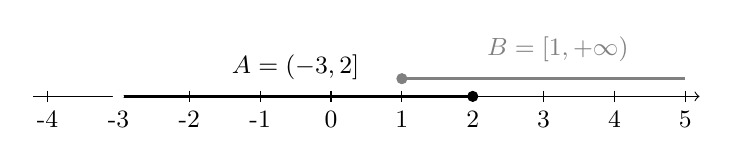
\begin{tikzpicture}[scale=0.9]
\draw[->] (-4.2,0) -- (5.2,0);
\foreach \x in {-4,-3,-2,-1,0,1,2,3,4,5}
  \draw (\x,0.08) -- (\x,-0.08) node[below] {\small \x};
\draw[line width=1.2pt] (-3,0) -- (2,0);
\filldraw[white] (-3,0) circle (2pt);
\filldraw[black] (2,0) circle (2pt);
\draw[line width=1.2pt, gray] (1,0.25) -- (5,0.25);
\filldraw[gray] (1,0.25) circle (2pt);
\node[above] at (-0.5,0.1) {\small \(A=(-3,2]\)};
\node[above, gray] at (3.2,0.35) {\small \(B=[1,+\infty)\)};
\end{tikzpicture}
\end{center}

\begin{solvedexample}{[EX-C01.S03-01] Escribir y combinar intervalos}
Sean
\[
A=\{x\in\mathbb{R}\mid -3<x\le 2\},
\qquad
B=\{x\in\mathbb{R}\mid x\ge 1\}.
\]
Escribe ambos conjuntos como intervalos y calcula \(A\cap B\) y \(A\cup B\).

\textbf{Desarrollo.}
\[
A=(-3,2],\qquad B=[1,+\infty).
\]
La parte comun va desde \(1\) hasta \(2\), ambos incluidos:
\[
A\cap B=[1,2].
\]
La union cubre desde \(-3\) sin incluir hasta \(+\infty\):
\[
A\cup B=(-3,+\infty).
\]
\end{solvedexample}

\begin{commonerror}{Confundir tocarse con estar separados}
Si un intervalo termina en \(5\) incluido y el siguiente empieza en \(5\) excluido, la union
sigue siendo un unico tramo. Hay contacto en el mismo punto.
\end{commonerror}

\begin{guidedexercise}{[GX-C01.S03-01] De desigualdad a intervalo}
Escribe en notacion de intervalos:
\[
x<-1 \quad \text{o} \quad x\ge 4.
\]
\end{guidedexercise}

\begin{shortanswer}{[GX-C01.S03-01]}
\[
(-\infty,-1)\cup [4,+\infty).
\]
\end{shortanswer}

\begin{fullsolution}{[GX-C01.S03-01]}
La desigualdad \(x<-1\) se escribe como \((-\infty,-1)\). La desigualdad \(x\ge 4\) se escribe
como \([4,+\infty)\). Como aparece ``o'', la respuesta final es la union:
\[
(-\infty,-1)\cup [4,+\infty).
\]
\end{fullsolution}

\begin{guidedexercise}{[GX-C01.S03-02] Interseccion de intervalos}
Calcula
\[
[-2,5)\cap (1,7].
\]
\end{guidedexercise}

\begin{shortanswer}{[GX-C01.S03-02]}
\[
(1,5).
\]
\end{shortanswer}

\begin{fullsolution}{[GX-C01.S03-02]}
Los valores comunes son los que estan a la vez entre \(-2\) y \(5\), y entre \(1\) y \(7\).
Por tanto:
\[
[-2,5)\cap (1,7]=(1,5).
\]
\end{fullsolution}

\subsection*{Practica autonoma graduada}
\begin{exercise}{[PX-C01.S03-01] Escribe en intervalos: \(x\le 3\) y \(x>-2\).}
\end{exercise}
\begin{exercise}{[PX-C01.S03-02] Calcula \((-\infty,1]\cap [1,4)\).}
\end{exercise}
\begin{exercise}{[PX-C01.S03-03] Calcula \([0,5]\cup (5,8)\).}
\end{exercise}
\begin{exercise}{[PX-C01.S03-04] Escribe en intervalos: \(x>2\).}
\end{exercise}
\begin{exercise}{[PX-C01.S03-05] Calcula \((-3,-1)\cap [-1,2]\).}
\end{exercise}
\begin{exercise}{[PX-C01.S03-06] Calcula \((-\infty,-2]\cup (-2,3)\).}
\end{exercise}

\begin{shortanswer}{C01.S03 practica autonoma}
\begin{enumerate}[label=\textbf{PX-C01.S03-\arabic*:}, leftmargin=*]
  \item \((-2,3]\)
  \item \(\{1\}\)
  \item \([0,8)\)
  \item \((2,+\infty)\)
  \item \(\varnothing\)
  \item \((-\infty,3)\)
\end{enumerate}
\end{shortanswer}

\begin{fullsolution}{C01.S03 practica autonoma}
\begin{enumerate}[label=\textbf{PX-C01.S03-\arabic*:}, leftmargin=*]
  \item ``y'' significa interseccion, asi que deben cumplirse ambas condiciones:
  \[
  (-2,3].
  \]
  \item El unico punto comun es \(1\), luego:
  \[
  (-\infty,1]\cap [1,4)=\{1\}.
  \]
  \item Como \(5\) ya esta incluido en el primer intervalo, la union es:
  \[
  [0,8).
  \]
  \item
  \[
  x>2 \Longleftrightarrow (2,+\infty).
  \]
  \item El primer intervalo no incluye \(-1\) y el segundo empieza en \(-1\), asi que no hay
  punto comun:
  \[
  \varnothing.
  \]
  \item Ambos tramos se tocan en \(-2\) y la union cubre todo hasta \(3\) sin incluirlo:
  \[
  (-\infty,3).
  \]
\end{enumerate}
\end{fullsolution}

\section{[C01.S04] Valor absoluto como distancia}

\subsection*{Objetivos de aprendizaje}
\begin{itemize}
  \item Interpretar \(|x-a|\) como distancia entre \(x\) y \(a\).
  \item Resolver ecuaciones e inecuaciones sencillas con valor absoluto.
\end{itemize}

\subsection*{Prerrequisitos}
\begin{itemize}
  \item Resolver ecuaciones e inecuaciones lineales.
\end{itemize}

\begin{theorybox}{Idea minima}
\[
|x-a|=d
\]
significa que \(x\) esta a distancia \(d\) del punto \(a\). Si \(d>0\), suele haber dos
soluciones:
\[
x-a=d \quad \text{o} \quad x-a=-d.
\]
\end{theorybox}

\begin{methodbox}{Como reconocer y resolver}
\begin{enumerate}
  \item Lee el valor absoluto como una distancia.
  \item Si es una ecuacion \(|u|=k\), plantea \(u=k\) y \(u=-k\).
  \item Si es una inecuacion \(|u|<k\), traduce a \(-k<u<k\).
\end{enumerate}
\end{methodbox}

\begin{solvedexample}{[EX-C01.S04-01] Ecuacion con dos soluciones}
Resuelve
\[
|2x-3|=5.
\]

\textbf{Desarrollo.} Planteamos los dos casos:
\[
2x-3=5
\qquad \text{o} \qquad
2x-3=-5.
\]
Del primero:
\[
2x=8 \Longrightarrow x=4.
\]
Del segundo:
\[
2x=-2 \Longrightarrow x=-1.
\]

\textbf{Respuesta final.}
\[
x=4 \quad \text{o} \quad x=-1.
\]
\end{solvedexample}

\begin{commonerror}{Olvidar la rama negativa}
Al resolver \(|u|=k\) con \(k>0\), no basta con imponer \(u=k\). Tambien hay que resolver
\(u=-k\).
\end{commonerror}

\begin{guidedexercise}{[GX-C01.S04-01] Dos puntos a la misma distancia}
Resuelve
\[
|x+1|=3.
\]
\end{guidedexercise}

\begin{shortanswer}{[GX-C01.S04-01]}
\[
x=2 \quad \text{o} \quad x=-4.
\]
\end{shortanswer}

\begin{fullsolution}{[GX-C01.S04-01]}
\[
x+1=3 \quad \text{o} \quad x+1=-3.
\]
Por tanto:
\[
x=2 \quad \text{o} \quad x=-4.
\]
\end{fullsolution}

\begin{guidedexercise}{[GX-C01.S04-02] Distancia menor que un numero}
Resuelve
\[
|x-2|<4.
\]
\end{guidedexercise}

\begin{shortanswer}{[GX-C01.S04-02]}
\[
-2<x<6.
\]
\end{shortanswer}

\begin{fullsolution}{[GX-C01.S04-02]}
\[
|x-2|<4 \Longleftrightarrow -4<x-2<4.
\]
Sumando \(2\) en los tres miembros:
\[
-2<x<6.
\]
\end{fullsolution}

\subsection*{Practica autonoma graduada}
\begin{exercise}{[PX-C01.S04-01] Resuelve \(|x|=7\).}
\end{exercise}
\begin{exercise}{[PX-C01.S04-02] Resuelve \(|3x-1|=2\).}
\end{exercise}
\begin{exercise}{[PX-C01.S04-03] Resuelve \(|x+4|\le 1\).}
\end{exercise}
\begin{exercise}{[PX-C01.S04-04] Halla los puntos cuya distancia a \(5\) es \(2\).}
\end{exercise}
\begin{exercise}{[PX-C01.S04-05] Resuelve \(|2x+3|>1\).}
\end{exercise}
\begin{exercise}{[PX-C01.S04-06] Resuelve \(|x-1|=0\).}
\end{exercise}

\begin{shortanswer}{C01.S04 practica autonoma}
\begin{enumerate}[label=\textbf{PX-C01.S04-\arabic*:}, leftmargin=*]
  \item \(x=\pm 7\)
  \item \(x=1\) o \(x=-\dfrac{1}{3}\)
  \item \([-5,-3]\)
  \item \(x=3\) o \(x=7\)
  \item \(x<-2\) o \(x>-1\)
  \item \(x=1\)
\end{enumerate}
\end{shortanswer}

\begin{fullsolution}{C01.S04 practica autonoma}
\begin{enumerate}[label=\textbf{PX-C01.S04-\arabic*:}, leftmargin=*]
  \item \(|x|=7\) equivale a \(x=7\) o \(x=-7\).
  \item
  \[
  3x-1=2 \quad \text{o} \quad 3x-1=-2.
  \]
  De ahi se obtiene \(x=1\) o \(x=-1/3\).
  \item
  \[
  |x+4|\le 1 \Longleftrightarrow -1\le x+4\le 1.
  \]
  Restando \(4\):
  \[
  -5\le x\le -3.
  \]
  \item Distancia \(2\) a \(5\) significa:
  \[
  |x-5|=2.
  \]
  Entonces \(x=7\) o \(x=3\).
  \item
  \[
  |2x+3|>1 \Longleftrightarrow 2x+3>1 \quad \text{o} \quad 2x+3<-1.
  \]
  Por tanto:
  \[
  x>-1 \quad \text{o} \quad x<-2.
  \]
  \item La unica distancia cero es el propio punto:
  \[
  x-1=0 \Longrightarrow x=1.
  \]
\end{enumerate}
\end{fullsolution}

\section{[C01.S05] Potencias y radicales}

\subsection*{Objetivos de aprendizaje}
\begin{itemize}
  \item Simplificar radicales y expresiones con potencias.
  \item Reconocer exponentes negativos y fraccionarios.
\end{itemize}

\subsection*{Prerrequisitos}
\begin{itemize}
  \item Reglas basicas de productos y cocientes.
\end{itemize}

\begin{theorybox}{Idea minima}
\[
a^{-n}=\frac{1}{a^n},
\qquad
a^{m/n}=\sqrt[n]{a^m}.
\]
Para sumar radicales, primero hay que simplificarlos hasta que tengan el mismo radical.
\end{theorybox}

\begin{methodbox}{Como reconocer y resolver}
\begin{enumerate}
  \item Aplica la propiedad correspondiente de potencias.
  \item Simplifica cada radical por separado.
  \item Suma o resta solo radicales semejantes.
\end{enumerate}
\end{methodbox}

\begin{solvedexample}{[EX-C01.S05-01] Radicales semejantes}
Simplifica
\[
\sqrt{50}-2\sqrt{8}+3\sqrt{18}.
\]

\textbf{Desarrollo.}
\[
\sqrt{50}=5\sqrt{2},\qquad \sqrt{8}=2\sqrt{2},\qquad \sqrt{18}=3\sqrt{2}.
\]
Entonces:
\[
\sqrt{50}-2\sqrt{8}+3\sqrt{18}=5\sqrt{2}-2(2\sqrt{2})+3(3\sqrt{2}).
\]
\[
=5\sqrt{2}-4\sqrt{2}+9\sqrt{2}=10\sqrt{2}.
\]

\textbf{Respuesta final.}
\[
\boxed{10\sqrt{2}}.
\]
\end{solvedexample}

\begin{commonerror}{Sumar radicales no semejantes}
No se puede pasar de \(\sqrt{8}+\sqrt{18}\) a \(\sqrt{26}\). Primero hay que simplificar cada
radical y despues operar solo si son semejantes.
\end{commonerror}

\begin{guidedexercise}{[GX-C01.S05-01] Exponente negativo}
Calcula
\[
2^3\cdot 2^{-5}.
\]
\end{guidedexercise}

\begin{shortanswer}{[GX-C01.S05-01]}
\[
\frac{1}{4}.
\]
\end{shortanswer}

\begin{fullsolution}{[GX-C01.S05-01]}
\[
2^3\cdot 2^{-5}=2^{3-5}=2^{-2}=\frac{1}{2^2}=\frac{1}{4}.
\]
\end{fullsolution}

\begin{guidedexercise}{[GX-C01.S05-02] Simplificar y sumar}
Calcula
\[
\sqrt{12}+\sqrt{27}.
\]
\end{guidedexercise}

\begin{shortanswer}{[GX-C01.S05-02]}
\[
5\sqrt{3}.
\]
\end{shortanswer}

\begin{fullsolution}{[GX-C01.S05-02]}
\[
\sqrt{12}=2\sqrt{3},\qquad \sqrt{27}=3\sqrt{3}.
\]
Por tanto:
\[
\sqrt{12}+\sqrt{27}=5\sqrt{3}.
\]
\end{fullsolution}

\subsection*{Practica autonoma graduada}
\begin{exercise}{[PX-C01.S05-01] Calcula \(3^{-2}\).}
\end{exercise}
\begin{exercise}{[PX-C01.S05-02] Simplifica \(\sqrt{75}-\sqrt{12}\).}
\end{exercise}
\begin{exercise}{[PX-C01.S05-03] Calcula \(16^{3/4}\).}
\end{exercise}
\begin{exercise}{[PX-C01.S05-04] Simplifica \(\dfrac{\sqrt[3]{54}}{\sqrt[3]{2}}\).}
\end{exercise}
\begin{exercise}{[PX-C01.S05-05] Simplifica \(\sqrt{45}+\sqrt{5}\).}
\end{exercise}
\begin{exercise}{[PX-C01.S05-06] Calcula \(\sqrt{2^4\cdot 5^2}\).}
\end{exercise}

\begin{shortanswer}{C01.S05 practica autonoma}
\begin{enumerate}[label=\textbf{PX-C01.S05-\arabic*:}, leftmargin=*]
  \item \(\dfrac{1}{9}\)
  \item \(3\sqrt{3}\)
  \item \(8\)
  \item \(3\)
  \item \(4\sqrt{5}\)
  \item \(20\)
\end{enumerate}
\end{shortanswer}

\begin{fullsolution}{C01.S05 practica autonoma}
\begin{enumerate}[label=\textbf{PX-C01.S05-\arabic*:}, leftmargin=*]
  \item
  \[
  3^{-2}=\frac{1}{3^2}=\frac{1}{9}.
  \]
  \item
  \[
  \sqrt{75}=5\sqrt{3},\qquad \sqrt{12}=2\sqrt{3},
  \]
  luego:
  \[
  \sqrt{75}-\sqrt{12}=3\sqrt{3}.
  \]
  \item
  \[
  16^{3/4}=\left(\sqrt[4]{16}\right)^3=2^3=8.
  \]
  \item
  \[
  \frac{\sqrt[3]{54}}{\sqrt[3]{2}}=\sqrt[3]{\frac{54}{2}}=\sqrt[3]{27}=3.
  \]
  \item
  \[
  \sqrt{45}=3\sqrt{5},
  \]
  asi que:
  \[
  \sqrt{45}+\sqrt{5}=4\sqrt{5}.
  \]
  \item
  \[
  \sqrt{2^4\cdot 5^2}=\sqrt{16\cdot 25}=\sqrt{400}=20.
  \]
\end{enumerate}
\end{fullsolution}

\section{[C01.S06] Racionalizacion}

\subsection*{Objetivos de aprendizaje}
\begin{itemize}
  \item Eliminar radicales del denominador.
  \item Usar conjugados cuando el denominador tiene dos terminos.
\end{itemize}

\subsection*{Prerrequisitos}
\begin{itemize}
  \item Productos notables sencillos.
\end{itemize}

\begin{theorybox}{Idea minima}
Si el denominador es un monomio radical, se multiplica arriba y abajo por el radical adecuado.
Si es un binomio con radical, suele usarse el conjugado:
\[
(a-b)(a+b)=a^2-b^2.
\]
\end{theorybox}

\begin{methodbox}{Como reconocer y resolver}
\begin{enumerate}
  \item Mira si el denominador tiene un solo radical o un binomio.
  \item Elige el factor que convierte el denominador en un numero sin radicales.
  \item Multiplica numerador y denominador por el mismo factor.
  \item Simplifica el resultado.
\end{enumerate}
\end{methodbox}

\begin{solvedexample}{[EX-C01.S06-01] Racionalizar con conjugado}
Racionaliza
\[
\frac{3}{\sqrt{5}-2}.
\]

\textbf{Desarrollo.} Multiplicamos por el conjugado:
\[
\frac{3}{\sqrt{5}-2}\cdot\frac{\sqrt{5}+2}{\sqrt{5}+2}
=\frac{3(\sqrt{5}+2)}{(\sqrt{5})^2-2^2}
=\frac{3(\sqrt{5}+2)}{5-4}.
\]
Por tanto:
\[
\frac{3}{\sqrt{5}-2}=3\sqrt{5}+6.
\]
\end{solvedexample}

\begin{commonerror}{Cambiar el denominador sin tocar el numerador}
Racionalizar no es ``modificar'' solo el denominador. Hay que multiplicar numerador y
denominador por el mismo factor para conservar la equivalencia.
\end{commonerror}

\begin{guidedexercise}{[GX-C01.S06-01] Monomio radical}
Racionaliza
\[
\frac{5}{\sqrt{2}}.
\]
\end{guidedexercise}

\begin{shortanswer}{[GX-C01.S06-01]}
\[
\frac{5\sqrt{2}}{2}.
\]
\end{shortanswer}

\begin{fullsolution}{[GX-C01.S06-01]}
\[
\frac{5}{\sqrt{2}}\cdot\frac{\sqrt{2}}{\sqrt{2}}=\frac{5\sqrt{2}}{2}.
\]
\end{fullsolution}

\begin{guidedexercise}{[GX-C01.S06-02] Conjugado con numerador uno}
Racionaliza
\[
\frac{1}{\sqrt{3}+\sqrt{2}}.
\]
\end{guidedexercise}

\begin{shortanswer}{[GX-C01.S06-02]}
\[
\sqrt{3}-\sqrt{2}.
\]
\end{shortanswer}

\begin{fullsolution}{[GX-C01.S06-02]}
\[
\frac{1}{\sqrt{3}+\sqrt{2}}\cdot\frac{\sqrt{3}-\sqrt{2}}{\sqrt{3}-\sqrt{2}}
=\frac{\sqrt{3}-\sqrt{2}}{3-2}
=\sqrt{3}-\sqrt{2}.
\]
\end{fullsolution}

\subsection*{Practica autonoma graduada}
\begin{exercise}{[PX-C01.S06-01] Racionaliza \(\dfrac{2}{\sqrt{7}}\).}
\end{exercise}
\begin{exercise}{[PX-C01.S06-02] Racionaliza \(\dfrac{4}{3-\sqrt{5}}\).}
\end{exercise}
\begin{exercise}{[PX-C01.S06-03] Racionaliza \(\dfrac{1}{2+\sqrt{3}}\).}
\end{exercise}
\begin{exercise}{[PX-C01.S06-04] Simplifica \(\dfrac{\sqrt{6}}{\sqrt{2}}\).}
\end{exercise}
\begin{exercise}{[PX-C01.S06-05] Racionaliza \(\dfrac{7}{\sqrt{7}-1}\).}
\end{exercise}
\begin{exercise}{[PX-C01.S06-06] Racionaliza \(\dfrac{3}{1-\sqrt{2}}\).}
\end{exercise}

\begin{shortanswer}{C01.S06 practica autonoma}
\begin{enumerate}[label=\textbf{PX-C01.S06-\arabic*:}, leftmargin=*]
  \item \(\dfrac{2\sqrt{7}}{7}\)
  \item \(3+\sqrt{5}\)
  \item \(2-\sqrt{3}\)
  \item \(\sqrt{3}\)
  \item \(\dfrac{7\sqrt{7}+7}{6}\)
  \item \(-3-3\sqrt{2}\)
\end{enumerate}
\end{shortanswer}

\begin{fullsolution}{C01.S06 practica autonoma}
\begin{enumerate}[label=\textbf{PX-C01.S06-\arabic*:}, leftmargin=*]
  \item
  \[
  \frac{2}{\sqrt{7}}\cdot\frac{\sqrt{7}}{\sqrt{7}}=\frac{2\sqrt{7}}{7}.
  \]
  \item
  \[
  \frac{4}{3-\sqrt{5}}\cdot\frac{3+\sqrt{5}}{3+\sqrt{5}}
  =\frac{4(3+\sqrt{5})}{9-5}=3+\sqrt{5}.
  \]
  \item
  \[
  \frac{1}{2+\sqrt{3}}\cdot\frac{2-\sqrt{3}}{2-\sqrt{3}}
  =\frac{2-\sqrt{3}}{4-3}=2-\sqrt{3}.
  \]
  \item
  \[
  \frac{\sqrt{6}}{\sqrt{2}}=\sqrt{\frac{6}{2}}=\sqrt{3}.
  \]
  \item
  \[
  \frac{7}{\sqrt{7}-1}\cdot\frac{\sqrt{7}+1}{\sqrt{7}+1}
  =\frac{7(\sqrt{7}+1)}{7-1}
  =\frac{7\sqrt{7}+7}{6}.
  \]
  \item
  \[
  \frac{3}{1-\sqrt{2}}\cdot\frac{1+\sqrt{2}}{1+\sqrt{2}}
  =\frac{3(1+\sqrt{2})}{1-2}
  =-3-3\sqrt{2}.
  \]
\end{enumerate}
\end{fullsolution}

\section{[C01.S07] Logaritmos y propiedades operativas}

\subsection*{Objetivos de aprendizaje}
\begin{itemize}
  \item Traducir entre expresion exponencial y logaritmica.
  \item Aplicar propiedades basicas de los logaritmos.
\end{itemize}

\subsection*{Prerrequisitos}
\begin{itemize}
  \item Potencias y exponentes.
\end{itemize}

\begin{theorybox}{Idea minima}
\[
\log_a b=c \Longleftrightarrow a^c=b.
\]
Ademas, para \(a>0\), \(a\neq 1\), \(x>0\), \(y>0\):
\[
\log_a(xy)=\log_a x+\log_a y,
\qquad
\log_a\left(\frac{x}{y}\right)=\log_a x-\log_a y.
\]
\end{theorybox}

\begin{methodbox}{Como reconocer y resolver}
\begin{enumerate}
  \item Si puedes, reescribe el logaritmo como una potencia conocida.
  \item Aplica propiedades solo cuando los argumentos sean positivos.
  \item Simplifica al final.
\end{enumerate}
\end{methodbox}

\begin{solvedexample}{[EX-C01.S07-01] Operar con logaritmos}
Calcula
\[
\log_3 81 + 2\log_3\left(\frac{1}{3}\right).
\]

\textbf{Desarrollo.}
\[
\log_3 81=4,
\qquad
\log_3\left(\frac{1}{3}\right)=-1.
\]
Entonces:
\[
\log_3 81 + 2\log_3\left(\frac{1}{3}\right)=4+2(-1)=2.
\]

\textbf{Respuesta final.}
\[
\boxed{2}.
\]
\end{solvedexample}

\begin{commonerror}{Olvidar que \(\log_a(1/a)=-1\)}
El logaritmo pregunta ``a que exponente hay que elevar la base''. Como
\[
a^{-1}=\frac{1}{a},
\]
se tiene \(\log_a(1/a)=-1\).
\end{commonerror}

\begin{guidedexercise}{[GX-C01.S07-01] Diferencia de logaritmos}
Calcula
\[
\log_2 32-\log_2 4.
\]
\end{guidedexercise}

\begin{shortanswer}{[GX-C01.S07-01]}
\[
3.
\]
\end{shortanswer}

\begin{fullsolution}{[GX-C01.S07-01]}
\[
\log_2 32=5,\qquad \log_2 4=2.
\]
Por tanto:
\[
\log_2 32-\log_2 4=5-2=3.
\]
\end{fullsolution}

\begin{guidedexercise}{[GX-C01.S07-02] Pasar a forma exponencial}
Resuelve
\[
\log_5 x=3.
\]
\end{guidedexercise}

\begin{shortanswer}{[GX-C01.S07-02]}
\[
x=125.
\]
\end{shortanswer}

\begin{fullsolution}{[GX-C01.S07-02]}
\[
\log_5 x=3 \Longleftrightarrow 5^3=x.
\]
Luego:
\[
x=125.
\]
\end{fullsolution}

\subsection*{Practica autonoma graduada}
\begin{exercise}{[PX-C01.S07-01] Calcula \(\log_{10}0.01\).}
\end{exercise}
\begin{exercise}{[PX-C01.S07-02] Calcula \(\log_4 64\).}
\end{exercise}
\begin{exercise}{[PX-C01.S07-03] Calcula \(\ln(e^5)\).}
\end{exercise}
\begin{exercise}{[PX-C01.S07-04] Calcula \(\log_2 8+\log_2 4\).}
\end{exercise}
\begin{exercise}{[PX-C01.S07-05] Calcula \(\log_3 27-\log_3 9\).}
\end{exercise}
\begin{exercise}{[PX-C01.S07-06] Resuelve \(\log_7 x=2\).}
\end{exercise}

\begin{shortanswer}{C01.S07 practica autonoma}
\begin{enumerate}[label=\textbf{PX-C01.S07-\arabic*:}, leftmargin=*]
  \item \(-2\)
  \item \(3\)
  \item \(5\)
  \item \(5\)
  \item \(1\)
  \item \(49\)
\end{enumerate}
\end{shortanswer}

\begin{fullsolution}{C01.S07 practica autonoma}
\begin{enumerate}[label=\textbf{PX-C01.S07-\arabic*:}, leftmargin=*]
  \item
  \[
  10^{-2}=0.01,
  \]
  luego \(\log_{10}0.01=-2\).
  \item
  \[
  4^3=64,
  \]
  asi que \(\log_4 64=3\).
  \item
  \[
  \ln(e^5)=5.
  \]
  \item
  \[
  \log_2 8+\log_2 4=3+2=5.
  \]
  \item
  \[
  \log_3 27-\log_3 9=3-2=1.
  \]
  \item
  \[
  \log_7 x=2 \Longleftrightarrow x=7^2=49.
  \]
\end{enumerate}
\end{fullsolution}

\begin{selfcheck}
\begin{itemize}
  \item Simplifico antes de clasificar un numero.
  \item Distingo entre decimal exacto, periodico puro y mixto.
  \item Manejo con seguridad intervalos, valor absoluto, radicales, racionalizacion y
  logaritmos basicos.
\end{itemize}
\end{selfcheck}

\begin{extension}{Puente al siguiente bloque}
El capitulo 2 retoma varias tecnicas de este bloque: simplificacion, equivalencia y control del
dominio. Esa continuidad es especialmente importante en fracciones algebraicas y ecuaciones
racionales.
\end{extension}
